\documentclass[11pt]{article}
%\usepackage{fullpage}
\usepackage[top=2cm, bottom=1.5cm, left=1.5cm, right=1.5cm]{geometry}
\usepackage{amsmath,amsthm,amsfonts,amssymb,amscd}
\usepackage{xcolor}
\usepackage{graphicx}
\usepackage[utf8]{inputenc}
\usepackage[english]{babel}
\usepackage{fancyhdr}
\usepackage{wrapfig}

\pagestyle{fancy}
\fancyhf{}
\fancyhead[LO]{Mechanics \& Relativity F3210}
\fancyhead[RO]{Workshop 7: Rotation}
%\fancyfoot[CE,CO]{\leftmark}
%\fancyfoot[LE,RO]{\thepage}

%answers
\usepackage{etoolbox}
\providetoggle{answers}
\settoggle{answers}{false}

\newcommand\vect[1]{\underline{\mathbf{#1}}}
\newcommand\unitvect[1]{\hat{\boldsymbol{#1}}}

\begin{document}

\noindent
\textbf{\textcolor{red}{Please upload your solution to Problem 3 to canvas for marking after the workshop.}}\\

\section*{Problem 1}

What is the angular speed (in radians per second) of the following components of the minute hand of a smoothly running analog watch?\\


\noindent

\section*{Problem 2}

In the figure below, wheel A of radius $r_A = 10$~cm is coupled by belt B to wheel C of radius $r_C = 25$ cm. The angular speed of wheel A is increased from rest at a constant rate of 1.6~rads$^{-2}$. Find the time needed for wheel C to reach an angular speed of 100 rev/min, assuming the belt does not slip. 

\begin{figure}[h]
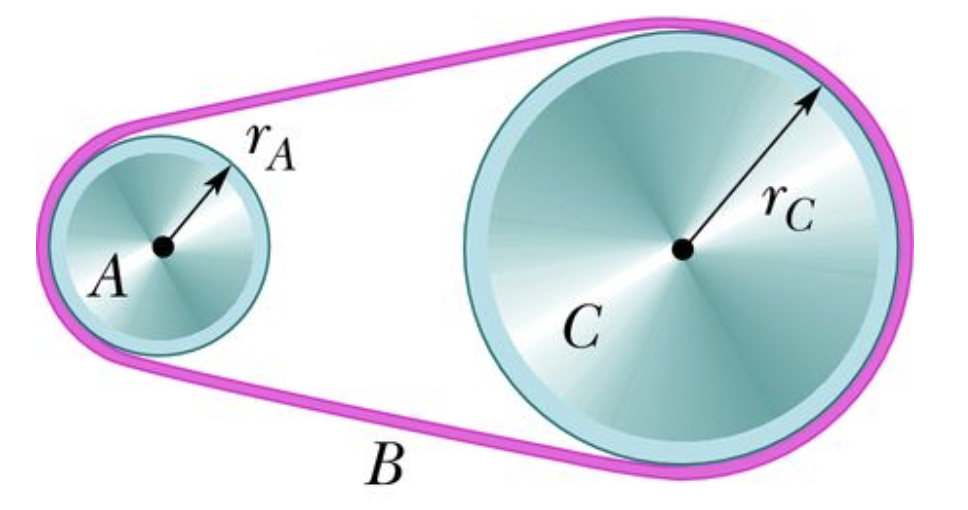
\includegraphics[scale=0.4]{2021-W7-Q2}

\end{figure}

\section*{\textcolor{red}{Problem 3}}
\fbox{\begin{minipage}{\textwidth}
A 0.400 kg ball is shot directly upward at initial speed 40.0 ms$^{-1}$. What is its angular momentum about P, 2.00 m horizontally from the launch point, when the ball is\\
 (a) at maximum height?\\
 (b) halfway back to the ground? \\
 What is the torque on the ball about P due to the gravitational force when the ball is \\
 (c) at maximum height?\\
 (d) halfway back to the ground?

\end{minipage}}


\section*{Problem 4}

A uniform solid sphere rolls down an incline. \\
(a) What must be the incline angle if the linear acceleration of the centre of the sphere is to have a magnitude of 0.10$g$? \\
(b) If a frictionless block were to slide down the incline at that angle, would its acceleration magnitude be more than, less than, or equal to 0.10$g$? Why?\\


%\vspace{0.5cm}
\section*{Want more practice?}
\small
Further problems on Angular Variables: Chapter 10.1-10.4 \\
Further problems on Inertia \& Torque: Chapter 10.5-10.8 \\
Further problems on Rolling \& Angular Momentum: Chapter 11\\
\end{document}





 




 


